%%%%%%%%%%%%%%%%%%%%%%%%%%%%%%%%%%%%%%%%%%%%%%%%%%%%%%%%%%%%%%%%%%%%%%%%%%%%%%%%%%%%%%
%%%%%%%%%%%%%%%%%%%%%%%%%%%%%%%%%%%%%%%%%%%%%%%%%%%%%%%%%%%%%%%%%%%%%%%%%%%%%%%%%%%%%%
%%%%%%%%%%%%%%%%%%%%%%%%%%%%%%%%%%%%%%%%%%%%%%%%%%%%%%%%%%%%%%%%%%%%%%%%%%%%%%%%%%%%%%
%% docART Utility - A Python/Lua(LaTeX) based tool for semi-automated documentation %%
%% Source: https://github.com/d-sacre/docart-documentation-utility/                 %%
%% Version: alpha-2022-04-30                                                        %%
%% License: GNU General Public License (GPLv3)                                      %%
%% Copyright (C) 2022 Martin Stimpfl, Daniel Sacré                                  %%
%%                                                                                  %%
%% This program is free software: you can redistribute it and/or modify             %%
%% it under the terms of the GNU General Public License as published by             %%
%% the Free Software Foundation, either version 3 of the License, or                %%
%% (at your option) any later version.                                              %%
%%                                                                                  %%
%% This program is distributed in the hope that it will be useful,                  %%
%% but WITHOUT ANY WARRANTY; without even the implied warranty of                   %%
%% MERCHANTABILITY or FITNESS FOR A PARTICULAR PURPOSE.  See the                    %%
%% GNU General Public License for more details.                                     %%
%%                                                                                  %%
%% You should have received a copy of the GNU General Public License                %%
%% along with this program.  If not, see <https://www.gnu.org/licenses/>.           %%
%%%%%%%%%%%%%%%%%%%%%%%%%%%%%%%%%%%%%%%%%%%%%%%%%%%%%%%%%%%%%%%%%%%%%%%%%%%%%%%%%%%%%%
%%%%%%%%%%%%%%%%%%%%%%%%%%%%%%%%%%%%%%%%%%%%%%%%%%%%%%%%%%%%%%%%%%%%%%%%%%%%%%%%%%%%%%
%%%%%%%%%%%%%%%%%%%%%%%%%%%%%%%%%%%%%%%%%%%%%%%%%%%%%%%%%%%%%%%%%%%%%%%%%%%%%%%%%%%%%%

\chapter{Configuration}
	\label{chap:config}
	\lstset{style=LaTeX}
	\section{\productName}
		After downloading and unpacking/cloning the \productName~github repository, the \productName~Utility is ready for use with the terminal/command line. However, one should do some clean-up and adapt it to ones' needs. To do so, open a file browser or terminal/command line and navigate to the folder where \productName~is located.
		\begin{enumerate}[label={\color{docartTurquoise}Step \arabic*:},leftmargin=*]
			\setlength\itemsep{-0.1em}
			\item In most cases it makes sense to delete the complete documentation source code in \mbox{\lstinline{./docart-utility/documentation/handbook_src/}}. Alternatively one can also simply delete the entire directory \mbox{\lstinline{./docart-utility/documentation/}}, which also removes the compiled pdf of the documentation.
			\item If one is not planning to use \lstinline{git} for version control, one can delete the \mbox{\lstinline{./.git/}-folder} and the \mbox{\lstinline{.gitignore}-file}. Otherwise, one should re-initialize the repository and adapt the \mbox{\lstinline{.gitignore}-file} to ones' requirements.
			\item One should rename the \lstinline{docart_mwe.tex} to a name representative for the intended use case, as the name of the compiled pdf file will be derived from the one of the main \LaTeX~file that gets compiled.
			\item Adjust the project setting files located at \mbox{\lstinline{./settings/}} (for details: see \mbox{section \ref{chap:adapting-default-theme}}). This is not necessary for the functionality and can be done at a later date. As long as these settings are not changed, the default values for \mbox{e.\,g.} \lstinline{\productName}, pdf author etc. will be used.
		\end{enumerate} 
	
	\vspace{-2.5cm}
	\section{TeXstudio}
		\label{sec:config:texstudio}
		For the usage with the \productName~Utility, the compilation options in TeXstudio have to be changed to provide shell escape functionality.
		\begin{daWarningBox}
			A TeXstudio compilation command containing shell escape is considered dangerous, as this setting is permanently present, even when not in use. This might enable attackers to execute malicious code.
			Please check whether permanent shell escape is compliant with your IT Security Policy before proceeding.
		\end{daWarningBox} 
		
		\newpage
		\begin{enumerate}[label={\color{docartTurquoise}Step \arabic*:},leftmargin=*]
			\item Start TeXstudio.
			\item Under \enquote{Options} select \enquote{Configure TeXstudio...}.\\[0.125cm]
			\begin{tikzpicture}
				\node[anchor=south west,inner sep=0] (image) at (0,0) {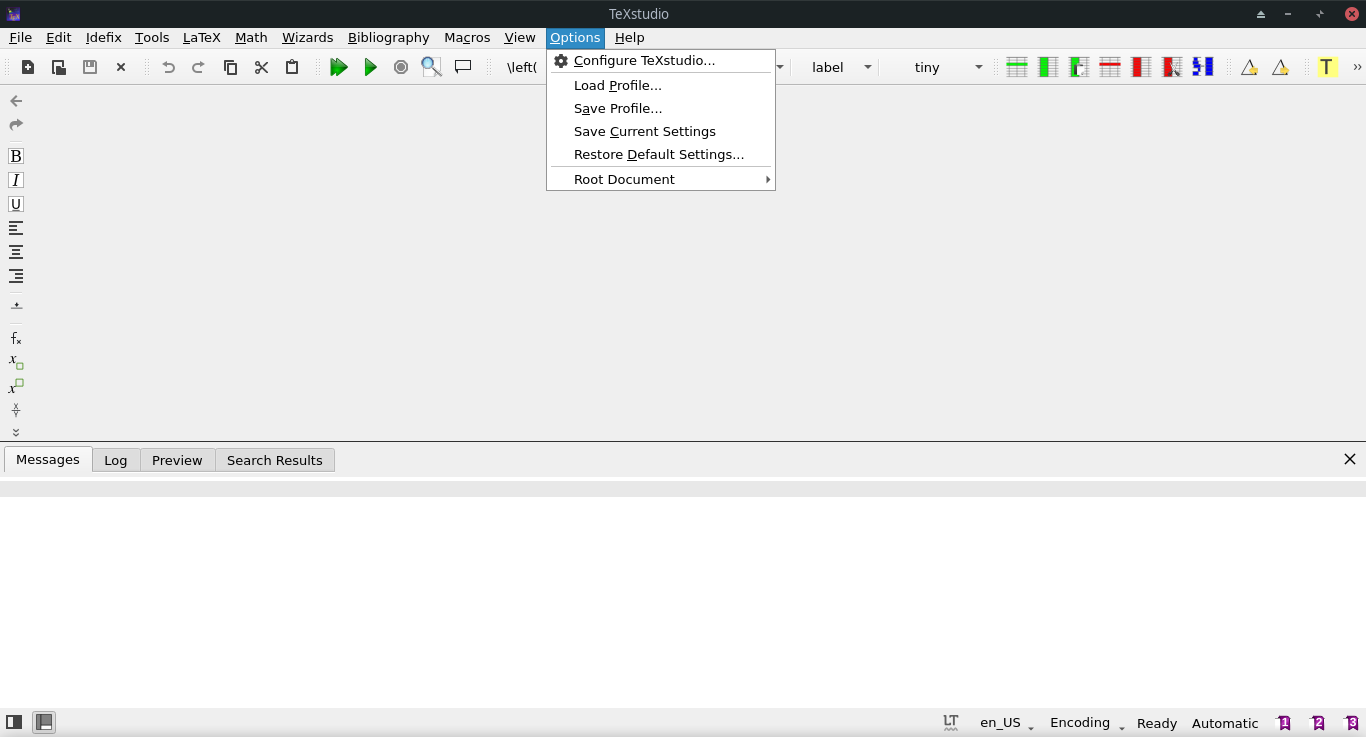
\includegraphics[width=0.75\linewidth]{./pictures/texstudio-config-screenshots/texstudio_options.png}};
				\begin{scope}[x={(image.south east)},y={(image.north west)}]
					\draw[orange,ultra thick](0.4,0.9)rectangle++(0.168,0.0325);
				\end{scope}
			\end{tikzpicture}
			\item Navigate to the \enquote{Command}-tab.\\[0.125cm]
			\begin{tikzpicture}
				\node[anchor=south west,inner sep=0] (image) at (0,0) {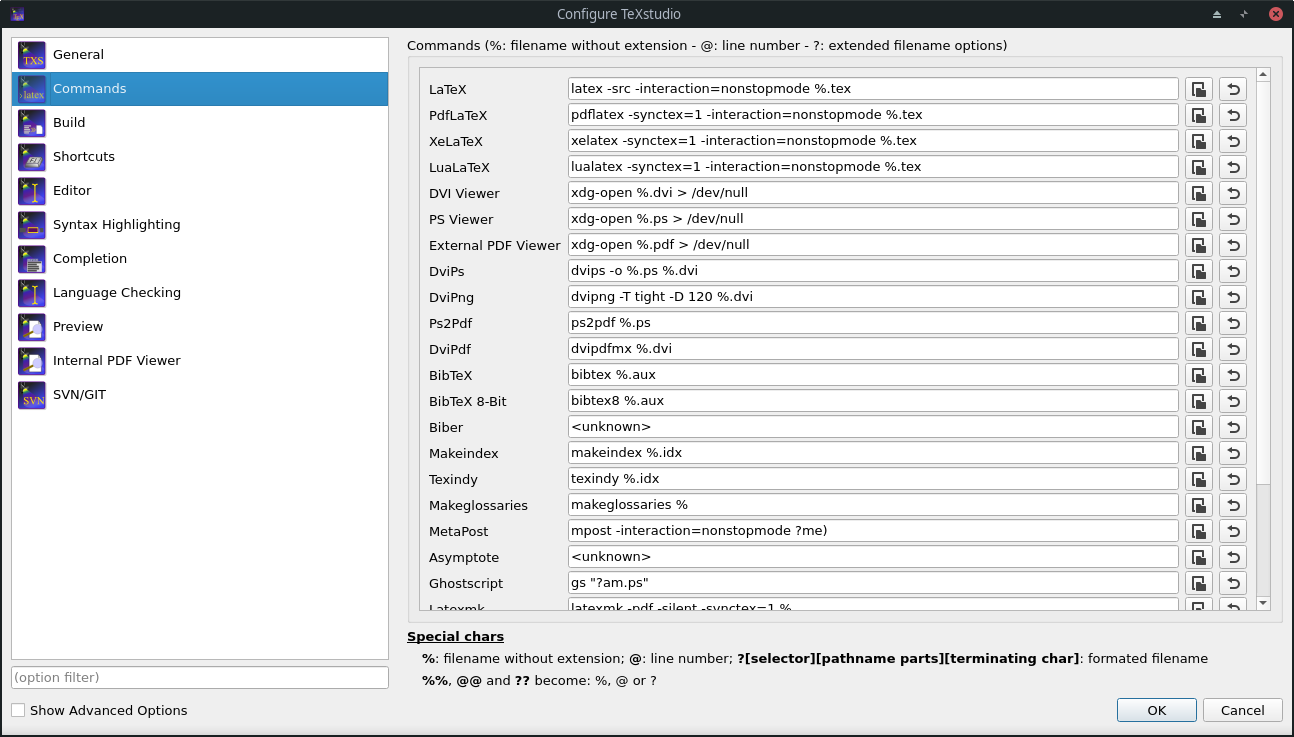
\includegraphics[width=0.75\linewidth]{./pictures/texstudio-config-screenshots/texstudio_commands.png}};
				\begin{scope}[x={(image.south east)},y={(image.north west)}]
					\draw[orange,ultra thick](0.0125,0.85)rectangle(0.3,0.9);
					\draw[orange,ultra thick](0.325,0.755)rectangle++(0.585,0.0325);
				\end{scope}
			\end{tikzpicture}
			\\[0.125cm]
			Replace the standard \enquote{LuaLaTeX}-entry\\[0.25cm]
			\lstinline$lualatex -synctex=1 -interaction=nonstopmode %.tex$
			\\[0.25cm]
			with:\\[0.25cm]
			\lstinline$lualatex --shell-escape -synctex=1 -interaction=nonstopmode %.tex$
			
			\item Confirm the changes by clicking on the \enquote{OK}-button. The changes will be applied and the configuration window will close.
		\end{enumerate}
		
	
	